%% Generator for UseCaseGuidance.pdf — the "which sort to reach for" strip chart.
%%
%% The figure was originally produced by matplotlib, whose script was not kept, so when the
%% measured crossovers moved there was no way to redraw it. This replaces that with TikZ, which
%% every LaTeX installation that can build the paper already has, so the figure is now source
%% rather than an artefact.
%%
%%   pdflatex UseCaseGuidance.tex
%%
%% Band edges come from the small-N crossover run (English corpus, JMH, 5 forks x 10 iterations)
%% reported in doc/Run results from Yunlu 2026-09-02.md:
%%
%%   N <= 20      System sort         (thin at 20: 0.462us against insertion sort's 0.489us)
%%   50 .. 200    insertion sort      wins outright
%%   500 .. 2000  QuickHuskySort
%%   >= ~10,000   RadixHuskySort      (its ~166us setup floor dominates below a few thousand)
%%
%% Solid where an algorithm wins outright; faded across the interval where the crossover falls,
%% since the measurements bracket each crossover rather than locating it exactly.

\documentclass[border=0pt]{standalone}
\usepackage{tikz}
\usetikzlibrary{shadings}
\usepackage{helvet}
\renewcommand{\familydefault}{\sfdefault}

\definecolor{bgpaper}{HTML}{FAF9F7}
\definecolor{cSystem}{HTML}{1F77B4}
\definecolor{cInsert}{HTML}{E2622A}
\definecolor{cQuick}{HTML}{2CA089}
\definecolor{cRadix}{HTML}{E8A317}

%% x is log10(N); one decade per \xunit
\newcommand{\xunit}{1.62cm}

\begin{document}
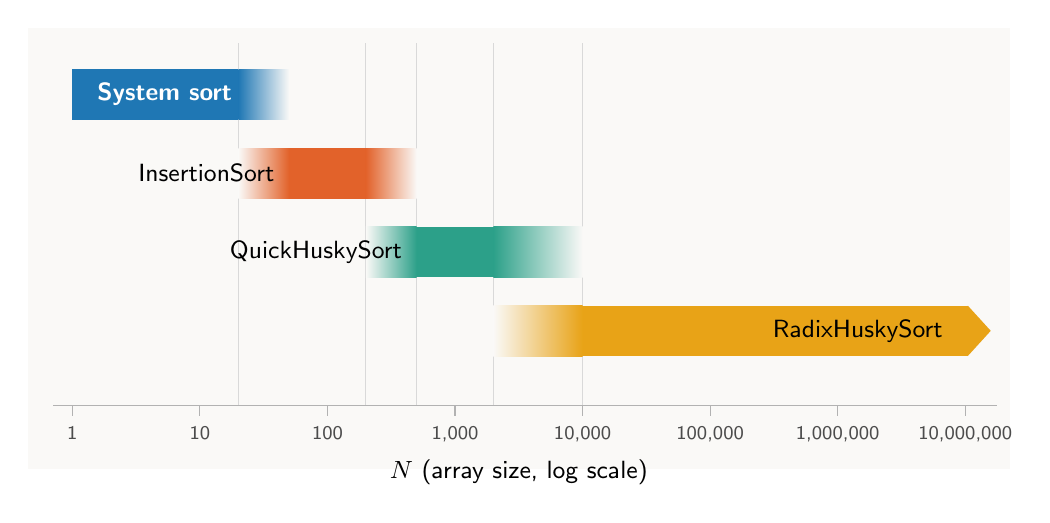
\begin{tikzpicture}[x=\xunit, y=1cm]

  %% ---- backdrop
  \fill[bgpaper] (-0.35,-1.25) rectangle (7.35,4.35);

  %% ---- vertical guides at the crossover decades
  \foreach \x in {1.301, 2.301, 2.699, 3.301, 4}
    \draw[gray!30, line width=0.4pt] (\x,-0.45) -- (\x,4.15);

  %% ---- bands.  #1 y-centre  #2 colour  #3 solid-from  #4 solid-to
  %%      fades are drawn as separate shaded rectangles either side.
  \newcommand{\band}[6]{%
    \fill[#2] (#3,#1-0.32) rectangle (#4,#1+0.32);
    \ifdim#5pt>0pt\relax
      \shade[left color=bgpaper, right color=#2] (#5,#1-0.32) rectangle (#3,#1+0.32);
    \fi
    \ifdim#6pt>0pt\relax
      \shade[left color=#2, right color=bgpaper] (#4,#1-0.32) rectangle (#6,#1+0.32);
    \fi
  }

  %% System sort: outright to N=20, fading out across 20..50
  \band{3.5}{cSystem}{0}{1.301}{0}{1.699}
  \node[anchor=west, text=white, font=\bfseries\small] at (0.12,3.5) {System sort};

  %% insertion sort: fading in across 20..50, outright 50..200, fading out across 200..500
  \band{2.5}{cInsert}{1.699}{2.301}{1.301}{2.699}
  \node[anchor=east, font=\small] at (1.66,2.5) {InsertionSort};

  %% QuickHuskySort: fading in across 200..500, outright 500..2000, fading out across 2000..10000
  \band{1.5}{cQuick}{2.699}{3.301}{2.301}{4}
  \node[anchor=east, font=\small] at (2.66,1.5) {QuickHuskySort};

  %% RadixHuskySort: fading in across 2000..10000, outright thereafter, open at the right
  \band{0.5}{cRadix}{4}{7.02}{3.301}{0}
  \node[anchor=east, font=\small] at (6.9,0.5) {RadixHuskySort};
  \fill[cRadix] (7.02,0.5-0.32) -- (7.02,0.5+0.32) -- (7.20,0.5) -- cycle;

  %% ---- axis
  \draw[gray!60, line width=0.6pt] (-0.15,-0.45) -- (7.25,-0.45);
  \foreach \x/\lab in {0/1, 1/10, 2/100, 3/1{,}000, 4/10{,}000,
                       5/100{,}000, 6/1{,}000{,}000, 7/10{,}000{,}000} {
    \draw[gray!60] (\x,-0.45) -- (\x,-0.58);
    \node[anchor=north, font=\scriptsize, text=black!70] at (\x,-0.60) {\lab};
  }
  \node[anchor=north, font=\small] at (3.5,-1.02) {$N$ (array size, log scale)};

\end{tikzpicture}
\end{document}
